\documentclass[12pt,a4paper,openright,twoside]{book}
\usepackage[utf8]{inputenc}
\usepackage{disi-thesis}
\usepackage{code-lstlistings}
\usepackage{notes}
\usepackage{shortcuts}
\usepackage{acronym}
\usepackage{svg}

\school{\unibo}
\programme{Corso di Laurea in Ingegneria e Scienze Informatiche}
\title{Sviluppo di un'Interfaccia Grafica per Software Simulativi Complessi mediante GraphQL e KotlinJS}
\author{Tiziano Vuksan}
\date{\today}
\subject{Programmazione ad Oggetti}
\supervisor{Dott. Danilo Pianini}
\cosupervisor{Dott. Angelo Filaseta}
\session{IV}
\academicyear{2023-2024}

% Definition of acronyms
%\acrodef{IoT}{Internet of Thing}
\acrodef{API}{Application Program Interface}
\acrodef{DOM}{Document Object Model}
\acrodef{REST}{Representational State Transfer}
\acrodef{URL}{Uniform Resource Identifier}
\acrodef{JVM}{Java Virtual Machine}


\mainlinespacing{1.241} % line spacing in mainmatter, comment to default (1)

\begin{document}

\frontmatter\frontispiece

\begin{abstract}	
Max 2000 characters, strict.
\end{abstract}

\begin{dedication} % this is optional
Optional. Max a few lines.
\end{dedication}

\begin{acknowledgements} % this is optional
Optional. Max 1 page.
\end{acknowledgements}

%----------------------------------------------------------------------------------------
\tableofcontents   
\listoffigures     % (optional) comment if empty
\lstlistoflistings % (optional) comment if empty
%----------------------------------------------------------------------------------------

\mainmatter

%----------------------------------------------------------------------------------------
%----------------------------------------------------------------------------------------
\chapter{Introduzione}
\label{chap:introduction}
%----------------------------------------------------------------------------------------

\section{Contesto}
\subsection{Simulazione}
\subsection{Alchemist}
\section{Motivazione}
\section{Obiettivi}
%----------------------------------------------------------------------------------------

%----------------------------------------------------------------------------------------
\chapter{Analisi}
%I suggest referencing stuff as follows: \cref{fig:random-image} or \Cref{fig:random-image}
%\begin{figure}
%	\centering
%	\includegraphics[width=.8\linewidth]{figures/random-image.pdf}
	%\caption{Some random image}
	%\label{fig:random-image}
%\end{figure}

\section{Requisiti}

Lo scopo principale del progetto è la realizzazione di una interfaccia web (quindi interpretabile da un qualsiasi browser moderno) che permetta l'interazione con il sistema software di simulazione
\textit{Alchemist} in modo intuitivo e \textit{user-friendly}. Il compito dell'applicativo sarà quindi quello di comunicare, attraverso apposite \ac{API}, con l'infrastruttura server preesistente e presentare in seguito a cambiamenti della simulazione in corso o a richieste da parte dell'utente, un'interfaccia grafica che ne rappresenti i risultati.
\subsection{Requisiti funzionali}
\begin{itemize}
	\item L'applicativo dovrà presentare un interfaccia grafica all'interno di un web browser.
	\item In una tipica simulazione di \textit{Alchemist} (come discusso nel paragrafo) sono presenti dei nodi. L'applicativo quindi dovrà essere in grado di rappresentare in un piano bidimensionale la posizione di tali nodi all'interno di un contesto grafico. Ciò implica ovviamente che con l'evolversi della simulazione il contesto grafico debba essere aggiornato. \footnote{Date le diverse \textit{incarnation} e i diversi possibili scenari che \textit{Alchemist} può modellare non è detto che i nodi cambino di posizione.}
	\item Ogni nodo contiene diverse proprietà, reazioni, concentrazioni etc. L'interfaccia dovrà permettere di ispezionare il contento di ciascun nodo. 
	\item L'interfaccia dovrà controllare lo stato attuale della simulazione. Ciò vuol dire poterla eseguire o mettere in pausa.
\end{itemize}

\subsection{Requisiti non funzionali}
\begin{itemize}
	\item Interagendo con l'interfaccia, non si devono verificare tempi di risposta eccessivi. Per esempio se l'utente decide di ispezionare un nodo, il recupero di tali informazioni deve essere presentato in tempi ragionevoli.
	\item  La comunicazione con l'infrastruttura server non deve impattare in modo negativo l'utilizzo dell'interfaccia stessa. 
	\item L'architettura delle componenti grafiche deve essere estendibile e facilmente 
\end{itemize}

\section{Analisi dei requisiti}

\section{Vincoli}

\section{Analisi e Modello del Dominio}

%----------------------------------------------------------------------------------------

%----------------------------------------------------------------------------------------
\chapter{Design}

%You may also put some code snippet (which is NOT float by default), eg: \cref{lst:random-code}.

%\lstinputlisting[float,language=Java,label={lst:random-code}]{listings/HelloWorld.java}

\section{Architettura generale client web}
In questa sezione viene esplorato come l'interfaccia web interagisce con le \ac{API} GraphQL per effettuare operazioni sul server e per poi usare i risultati di suddette operazioni per mostrarli graficamente. Nella figura \ref{fig:general-client-architecture-graphics} vengono mostrate le principali componenti protagoniste di questo meccanismo. Le descriviamo in questo modo:

 \begin{itemize}
	\item \textbf{Client Application}: questo \textit{package} contiene tutte le componenti grafiche che vengono rappresentate all'interno della pagina principale. Ogni componente, una volta che l'applicativo viene avviato, è tradotto al browser in formato HTML.
	\item \textbf{ClientConnection}: punto di accesso attraverso il quale è possibile effettuare tutte le operazioni definite secondo lo schema GraphQL. 
	\item \textbf{SimulationControlApi}: questo oggetto contiene tutte le funzioni necessarie a controllare lo stato della simulazione e dipende strettamente dalla componente \textbf{ClientConnection}. Si parla quindi di funzioni utili all'avvio, alla sospensione e terminazione della simulazione. Notare come queste siano tutte operazioni di tipo \textit{mutation}.
	\item \textbf{EnvironmentApi}: è l'oggetto utile a recuperare le informazioni riguardanti un nodo, lo stato \textit{attuale} dell'\textit{Environment}, ma soprattutto utile a recuperare la posizione dei nodi in tempo reale, quindi attraverso l'utilizzo di una \textit{subscription}. 
	\item \textbf{GeneratedModel}: questo pacchetto contiene tutte le risorse generate a partire dallo schema GraphQL esposto dal server. È utilizzato dagli oggetti \textbf{EnvironmentApi} e \textbf{SimulationControlApi} nell'utilizzo dei tipi di dato corretto durante l'utilizzo delle operazioni sul server.
 \end{itemize}

\begin{figure}[htb]
	\centering
	\includegraphics[scale=0.5]{imgs/General_Architecture_Web_Client.pdf}
	\caption{Architettura generale del client web}
	\label{fig:general-client-architecture-graphics}
\end{figure}

Gli oggetti \textbf{SimulationControlApi} e \textbf{EnvironmentApi} sono stati implementati attraverso il design pattern \textit{Singleton}~\cite{Gamma1994}. Sebbene quest'ultimo, se abusato o implementato in modo non adeguato sia considerato di fatto un ``anti-pattern'' \footnote{\url{https://code.google.com/archive/p/google-singleton-detector/wikis/WhySingletonsAreControversial.wiki}}, in questa situazione risulta essere molto comodo, specialmente considerando la necessità di un unico punto di accesso comune al client che effettua le query sul server. Risulterebbe infatti inutile, per ogni componente grafico che ne necessita, istanziare un'altro client GraphQL dal quale effettuare query. Lo stesso vale anche nell'ipotesi in cui vengano utilizzate delle proprietà che fungono da parametri di configurazione dell'applicativo. Un \textit{Singleton} può fornire un punto centralizzato per queste impostazioni.

\section{}


\section{Layout dell'interfaccia}
Il layout dell'interfaccia grafica è stato pensato per rappresentare nel modo più semplice ed intuitivo l'ambiente della simulazione.  La figura \ref{fig:interface-layout} rappresenta un mockup utilizzato durante la fase di progettazione dell'interfaccia. Si possono individuare le seguenti sezioni:
\begin{itemize}
	\item \textbf{Barra di navigazione}: nella parte alta dell'interfaccia è presente una barra di navigazione contenente il titolo e il pulsante per avviare o mettere in pausa la simulazione, ancorato all'estrema destra. Molte interfacce web moderne presentano questo tipo di elemento come \textit{header} della pagina web principale, inteso come punto centrale dal quale è possibile accedere a tutte le sezioni e funzionalità. Questo fornisce all'interfaccia un punto di espandibilità dell'applicativo, come l'aggiunta di una barra di ricerca o di un menù `detto ad `hamburger''. Sarebbe stato possibile, per esempio, inserire una barra di ricerca per i nodi, filtrandoli per categorie di proprietà. Questo tipo di funzionalità è indirizzato a lavori futuri. 
	\item \textbf{Canvas grafico}: la sezione principale di questa interfaccia. All'interno di un contesto grafico bidimensionale vengono rappresentati i nodi della simulazione. Ogni nodo è rappresentato come un cerchio pieno, avente centro le coordinate del nodo e raggio un valore variabile che può essere impostato dall'utente nella sezione descritta successivamente. Lo spazio bidimensionale ha come sfondo una griglia, che  fornisce un riferimento visivo e un aiuto all'orientamento. Funzionalità non banale di questa sezione è che l'utente può spostare il contesto visivo trascinando il cursore sullo schermo, oltre che a effettuare un ingrandimento o una diminuzione della scala. Per ottenere questo tipo di comportamenti sono stati adottati meccanismi ad hoc per il calcolo dello spostamento del \textit{drag} e dello \textit{zoom-in}/\textit{zoom-out}.
	\item \textbf{Informazioni e controlli sul canvas}: in questa sezione vengono raccolte le principali informazioni riguardo al contesto come il fattore di \textit{zoom} corrente, la differenza di traslazione rispetto all'origine e lo \textit{slider} per il cambiamento del raggio dei nodi.
	\item \textbf{Sezione di ispezione di un nodo}: qui vengono rappresentate tutte le informazioni riguardanti un nodo. Sono presenti quindi il codice identificativo, posizione nello spazio bidimensionale, proprietà, i contenuti (intesi come una mappa che ha come chiavi le molecole e  valori le relative concentrazioni), e le reazioni (Vedi \ref{label}). Per le ultime tre categorie sono stati usati degli elementi che possono essere ``collassati'' in quanto non è garantito che queste proprietà siano presenti (sempre per il fatto che \textit{Alchemist} può rappresentare una certa gamma di simulazioni tra loro eterogenee).
\end{itemize}

\begin{figure}[htb]
	\centering
	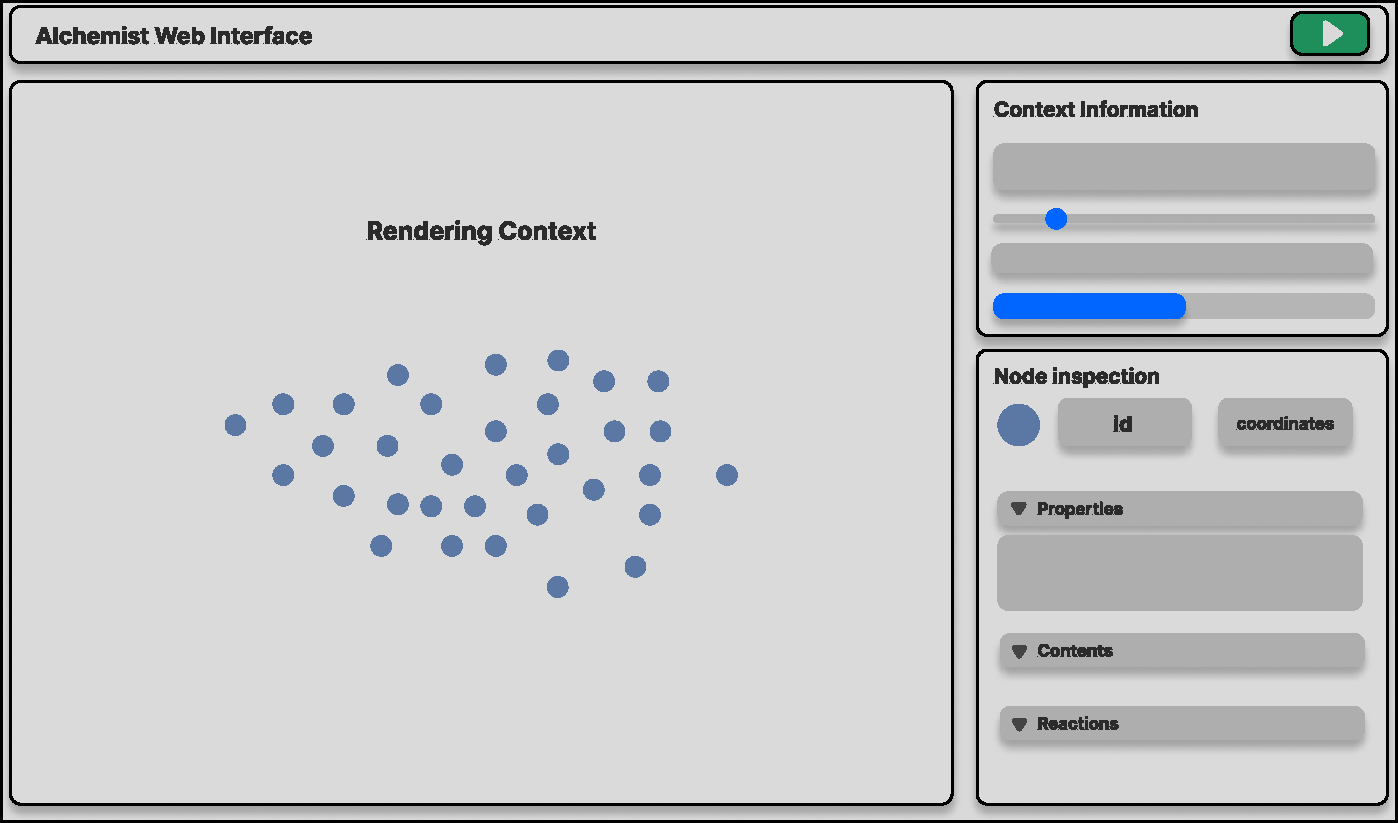
\includegraphics[scale=0.65]{imgs/Interface_Layout.pdf}
	\caption{Mockup dell'interfaccia grafica}
	\label{fig:interface-layout}
\end{figure}


%----------------------------------------------------------------------------------------

%----------------------------------------------------------------------------------------
\chapter{Implementazione e Verifica}

\section{Componenti grafici}

\section{Uso di Redux}

\section{State binding}

\section{Integrazioni di operazioni GraphQL}

\section{Verifica}
%----------------------------------------------------------------------------------------

%----------------------------------------------------------------------------------------
%!TEX root = ./thesis-main.tex
\chapter{Conclusione}
La totalità delle considerazioni e delle tecniche di sviluppo affrontate in questo documento ha portato alla creazione di una interfaccia web capace di rappresentare correttamente l'ambiente delle simulazioni di Alchemist, facendo uso delle \ac{API} GraphQL e utilizzando come linguaggio di sviluppo KotlinJS. Questo ha permesso di usare tecnologie coerenti alla \textit{codebase} esistente, evitando di usare stack tecnologici incompatibili che ne avrebbero potuto complicare l'integrazione. Il lavoro compiuto ha portato alla creazione di un prodotto allineato con le esigenze e gli obiettivi del progetto. 
Si è fatto impiego di strumenti, tra cui librerie e framework popolari, che godono di un continuo supporto in termini di aggiornamenti e correzioni da parte di una community attiva. L'utilizzo di tali risorse ha agevolato il processo di sviluppo e fornito una solida base su cui costruire e ampliare il prodotto.
È importante far notare come il risultato finale, allo stato attuale, non rappresenta il completo funzionamento del sistema, principalmente a causa della stretta dipendenza dalle \ac{API} fornite. Questa dipendenza limita la capacità di rappresentare tutte le potenzialità del sistema. Inoltre, per rispettare i requisiti iniziali nelle tempistiche a disposizione, si è dovuto utilizzare solo un sottoinsieme delle possibili interrogazioni, il che, di conseguenza, risulta in rappresentazioni limitate. In ogni caso, questo progetto fornisce un punto di partenza per l'espansione delle funzionalità e il miglioramento delle rappresentazioni future. Alcune di queste sono esplorate nella sezione successiva.

A titolo di esempio, vengono presentati due casi illustrativi.

Nella \cref{fig:protelis-example} si osserva l'interfaccia grafica che mostra una simulazione in esecuzione con l'incarnation \textit{protelis}\footnote{\url{https://alchemistsimulator.github.io/reference/yaml/}}. In questa configurazione, gli agenti cognitivi sono incaricati di evitare una zona pericolosa mentre si dirigono verso un obiettivo. Gli agenti si possono spingere tra di loro, creando variazioni uniche a ogni esecuzione.
\begin{figure}
	\centering
	\includegraphics[scale=0.22]{imgs/screens/example_protelis.png}
	\caption{Esempio di simulazione tramite l'incarnation protelis}
	\label{fig:protelis-example}
\end{figure}
\begin{figure}
	\centering
	\includegraphics[scale=0.22]{imgs/screens/example_sapere.png}
	\caption{Esempio di simulazione tramite l'incarnation sapere}
	\label{fig:sapere-example}
\end{figure}

Nella \cref{fig:sapere-example} è riportata invece l'esecuzione di una simulazione con l'incarnation \textit{sapere}\footnote{\url{https://alchemistsimulator.github.io/tutorials/basics/}}. Questa configurazione raffigura un processo di diffusione di un gradiente all'interno di una griglia di nodi a partire da una sorgente. Gli agenti nella simulazione interagiscono seguendo regole specifiche che influenzano la propagazione del gradiente in base alla loro posizione e al valore del gradiente nelle celle circostanti. 
Nel caso fosse supportata graficamente l'effettistica che mostrerebbe il gradiente, si renderebbe visibile il cambiamento di colori dei singoli nodi al variare del processo di propagazione definito. Tuttavia, per gli stessi motivi menzionati in precedenza, questa funzionalità è rimandata a lavori futuri.

\section{Lavori futuri}
Esistono diverse direzioni che potrebbero essere esplorate per migliorare ulteriormente l'interfaccia. Di seguito ne vengono elencate alcune:

\begin{itemize}
	\item \textbf{Rappresentazioni e interazioni aggiuntive}: la varietà delle operazioni possibili sullo \textit{schema} tramite il server GraphQL permette di ottenere dati che possono essere presentati all'utente in diversi modi. Come già menzionato in precedenza, è stata utilizzata una parte delle interrogazioni possibili. Alcune idee riguardanti a questo tipo di lavori può includere:
	\begin{itemize}
		\item Aggiunta di una barra di ricerca. Potrebbe essere utile cercare i nodi per codice identificativo (oppure per qualche altro criterio sensato), fornendo una lista di risultati che può essere raggruppata per \textbf{neighborhood} di appartenenza o per proprietà. \label{item:research-bar}
		\item Rappresentazione grafica delle \textbf{linking rule}. Non appena una implementazione da parte del modulo backend \texttt{graphql} permetterà di ottenere una struttura dati che definisce le linking rule fra i nodi, sarebbe opportuno fornirne una rappresentazione grafica. 
		\item Rappresentazione grafica dei \textbf{layers}. Un ``layer'' è un strato o sovrapposizione di dati che modella proprietà fisiche come inquinamento, luce, temperatura, e così via. 
		\item Visualizzazione del \textbf{neighborhood} di appartenenza. Al momento questo tipo di informazione non è disponibile all'interno dell'ispezione del nodo. Sarebbe auspicabile se al click su un nodo si evidenziassero graficamente i nodi appartenenti al vicinato.
	\end{itemize}
	\item \textbf{Aggiunta di feedback sulle operazioni utente}: un feedback visivo sullo stato delle operazioni, specialmente se falliscono, sarebbe un punto a favore per l'interfaccia in termini di esperienza d'uso. Questo feedback può assumere diverse forme, come conferme visive tramite pop-up, messaggi di stato, animazioni o suoni. Un feedback efficace fornisce all'utente informazioni chiare e tempestive sulle azioni che sta eseguendo, confermando il successo o l'errore dell'operazione eseguita.
	\item \textbf{Esperienza personalizzata}: potrebbe essere gradita l'implementazione di un sistema di salvataggio di preferenze personali come tema (chiaro/scuro), grandezza del font, la memorizzazione della disposizione delle sezioni grafiche principali in layout predefiniti o personalizzati etc.
	\item \textbf{Supporto all'effettistica}: all'interno delle interfacce desktop già esistenti per Alchemist, è possibile fornire al sistema un file di configurazione che definisce l'aspetto delle varie entità e descrive come tale aspetto deve cambiare in funzione della simulazione. Per equiparare l'interfaccia web alle interfacce già esistenti in termini di funzionalità, sarà necessario implementare questa caratteristica nell'interfaccia grafica futura. L'integrazione di questo aspetto è fondamentale poiché completa la rappresentazione grafica del modello di simulazione, considerando che diverse simulazioni fanno proprio uso di questo meccanismo.
	\item \textbf{Profiling delle prestazioni}: attualmente, l'interfaccia grafica presenta casi di \textit{stuttering} nel caso vengano configurate simulazioni con una quantità considerevole di nodi. La ricerca della sorgente di questo problema risulterebbe semplificata se si facesse ricorso a un processo di \textit{profiling}. Quest'ultimo implica l'analisi approfondita delle prestazioni dell'interfaccia utente al fine di identificare le aree di inefficienza o di degrado delle prestazioni. Attraverso questo sistema, sarà possibile individuare i punti critici dell'applicazione web, come tempi di caricamento prolungati, esecuzione di operazioni computazionalmente intensive o utilizzo eccessivo delle risorse di sistema. Queste informazioni saranno fondamentali per ottimizzare il codice, migliorare l'efficienza dell'interfaccia e garantire un'esperienza utente fluida e reattiva.
\end{itemize}
%----------------------------------------------------------------------------------------

%----------------------------------------------------------------------------------------
% BIBLIOGRAPHY
%----------------------------------------------------------------------------------------

\backmatter

\nocite{*} % comment this to only show the referenced entries from the .bib file

%\bibliographystyle{alpha}
%\bibliography{bibliography}

\end{document}